\documentclass{article}
\usepackage{tikz}
\usetikzlibrary{positioning, backgrounds, shapes.geometric, arrows.meta}
\begin{document}
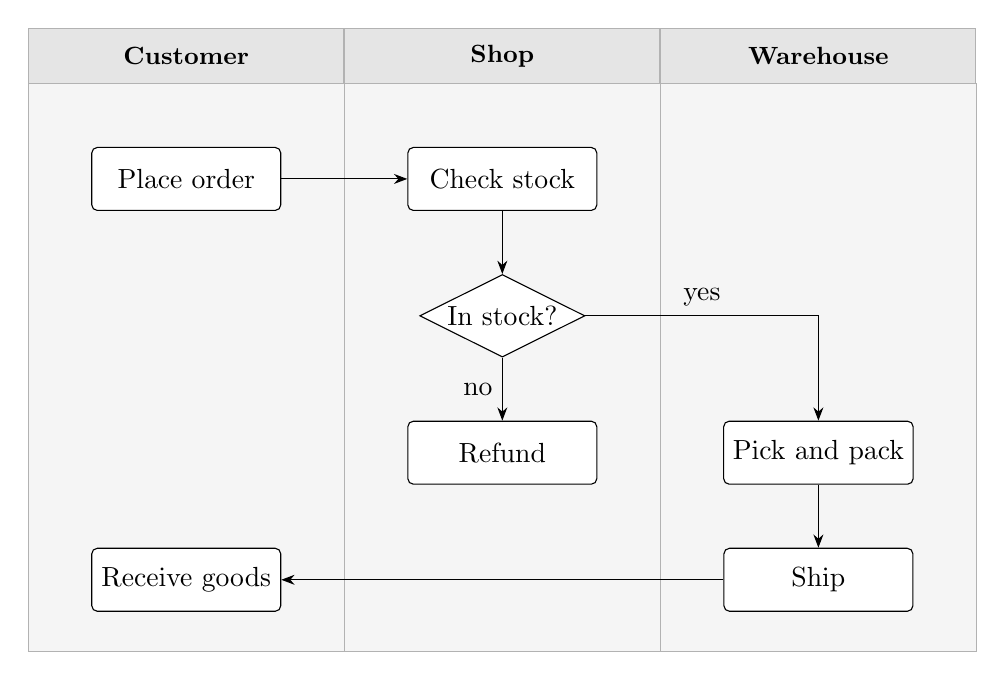
\begin{tikzpicture}[node distance=8mm and 16mm, >=Stealth,
  process/.style={draw, rounded corners=2pt, fill=white, minimum width=24mm, minimum height=8mm, align=center},
  decision/.style={draw, diamond, aspect=2, fill=white, inner sep=1pt, align=center},
  lane header/.style={draw=gray!60, fill=gray!20, minimum width=40mm, minimum height=7mm, font=\bfseries\small},
  lane/.style={draw=gray!60, fill=gray!8}]
  % Lanes: a header each, side by side; every node sits under its lane's header.
  \node[lane header] (customer) {Customer};
  \node[lane header, right=0pt of customer] (shop) {Shop};
  \node[lane header, right=0pt of shop] (warehouse) {Warehouse};

  \node[process, below=of customer] (order) {Place order};
  \node[process, below=of shop] (check) {Check stock};
  \node[decision, below=of check] (instock) {In stock?};
  \node[process, below=of instock] (refund) {Refund};
  \node[process] (pick) at (warehouse |- refund) {Pick and pack};
  \node[process, below=of pick] (ship) {Ship};
  \node[process] (receive) at (customer |- ship) {Receive goods};

  \draw[->] (order) -- (check);
  \draw[->] (check) -- (instock);
  \draw[->] (instock) -- node[auto, swap] {no} (refund);
  \draw[->] (instock) -| node[auto, pos=0.25] {yes} (pick);
  \draw[->] (pick) -- (ship);
  \draw[->] (ship) -- (receive);

  % The lanes run from their header down past the lowest node.
  \begin{scope}[on background layer]
    \draw[lane] (customer.south west) rectangle ([yshift=-5mm]customer.east |- receive.south);
    \draw[lane] (shop.south west) rectangle ([yshift=-5mm]shop.east |- receive.south);
    \draw[lane] (warehouse.south west) rectangle ([yshift=-5mm]warehouse.east |- receive.south);
  \end{scope}
\end{tikzpicture}
\end{document}
